\documentclass{article}

\usepackage{polski}
\usepackage[utf8]{inputenc}
\usepackage{graphicx}
\graphicspath{ {images/} }

\usepackage{float}
\usepackage{amsmath}
\usepackage{geometry} 

\author{Jakub Postępski}
\title{STP - Projekt I, zadanie 23}
\begin{document}
\maketitle

Obiekt opisany jest transmitancją ciągłą
\[ G(s) = \frac{(s+0.5)(s+3.5)}{(s-6)(s+4)(s+5)} \]
\section{Zadanie 1 - Wyznaczanie modelu w przestrzeni stanów}
Z prostych przekształceń mamy:
\[ G(s) = \frac{s^2 + 4s + 1.75}{s^3 + 3s^2 -34s -120)} = \frac{s^{-1} + 4s^{-2} + 1.75s^{2}}{1 + 3s^{-1} -34s^{-2} -120s^{-3})} = \frac{Y(s)}{U(s)}\]

Przyjmujemy pomocniczy:
\[E(s) = \frac{U(s)}{1 + 3s^{-1} -34s^{-2} -120s^{-3})} = U(s) - 3s^{-1}+34s^{-2} + 120s^{-3}\]
Dodatkowo:
\[Y(s) = (s^{-1} + 4s^{-2} + 1.75s^{2})E(s)\]

Dlatego model (pierwszy wariant metody bezpośredniej, rys. \ref{fig:z11}) w reprezentacji macierzowej:
\[A_1 = \begin{bmatrix} -3 & 34 & 120\\ 1 & 0 & 0\\ 0 & 1 & 0 \end{bmatrix};
B_1 = \begin{bmatrix} 1\\ 0\\ 0 \end{bmatrix};
C_1 = \begin{bmatrix} 1 & 4 & 1.75 \end{bmatrix};
D_1 = 0
\]
\begin{figure}
\centering
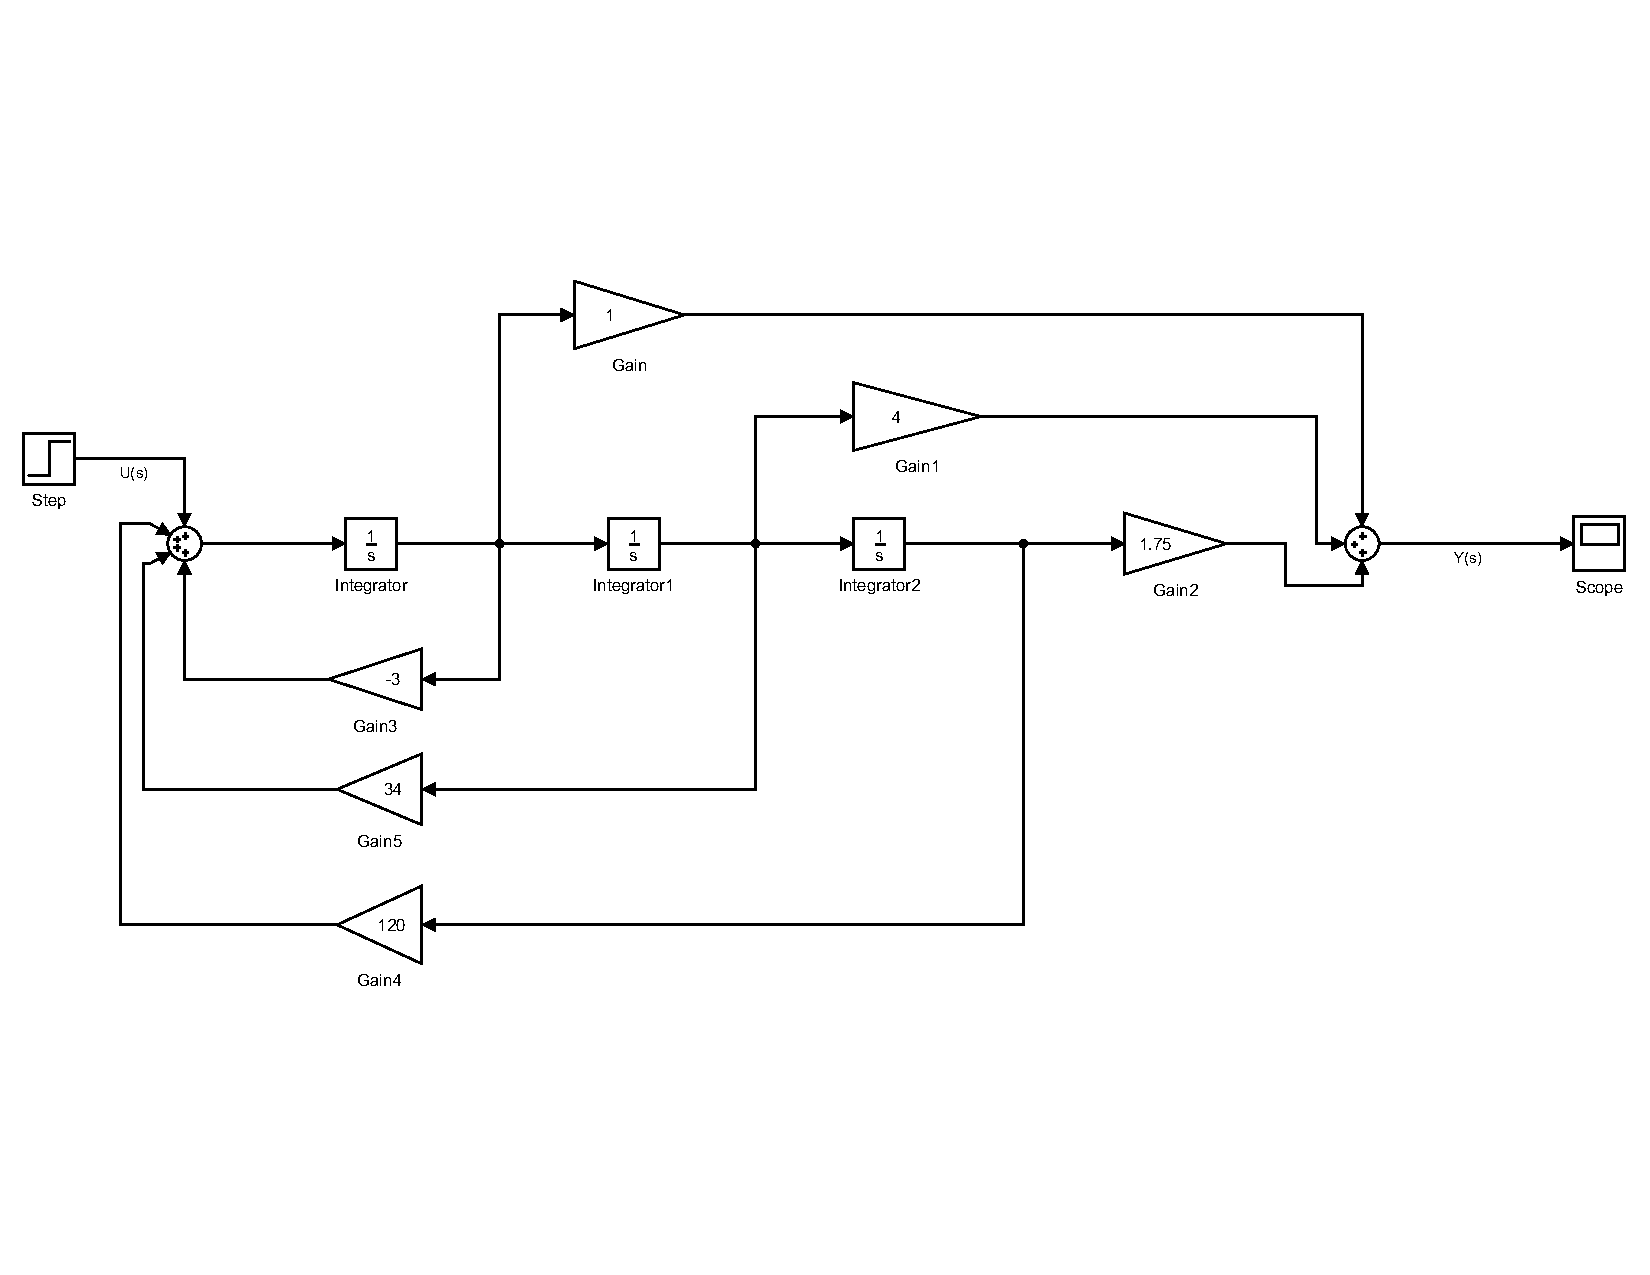
\includegraphics[width=0.9\linewidth]{z1_1}
\caption{Reprezentacja graficzna modelu otrzymanego pierwszym wariantem metody bezpośredniej}
\label{fig:z11}
\end{figure}

Reprezentacje wariantu drugiego metody bezpośredniej (rys. \ref{fig:z12}) otrzymujemy z zależności:
\[A_2 = A_1^T = \begin{bmatrix} -3 & 1 & 0\\ 34 & 0 & 1\\ 120 & 0 & 0 \end{bmatrix};
B_2 = C_1^T = \begin{bmatrix}  1\\ 4\\ 1.75 \end{bmatrix};
C_2 = B_1^T = \begin{bmatrix} 1 & 0 & 0 \end{bmatrix};
D_2 = D_1 = 0
\]
\begin{figure}
\centering
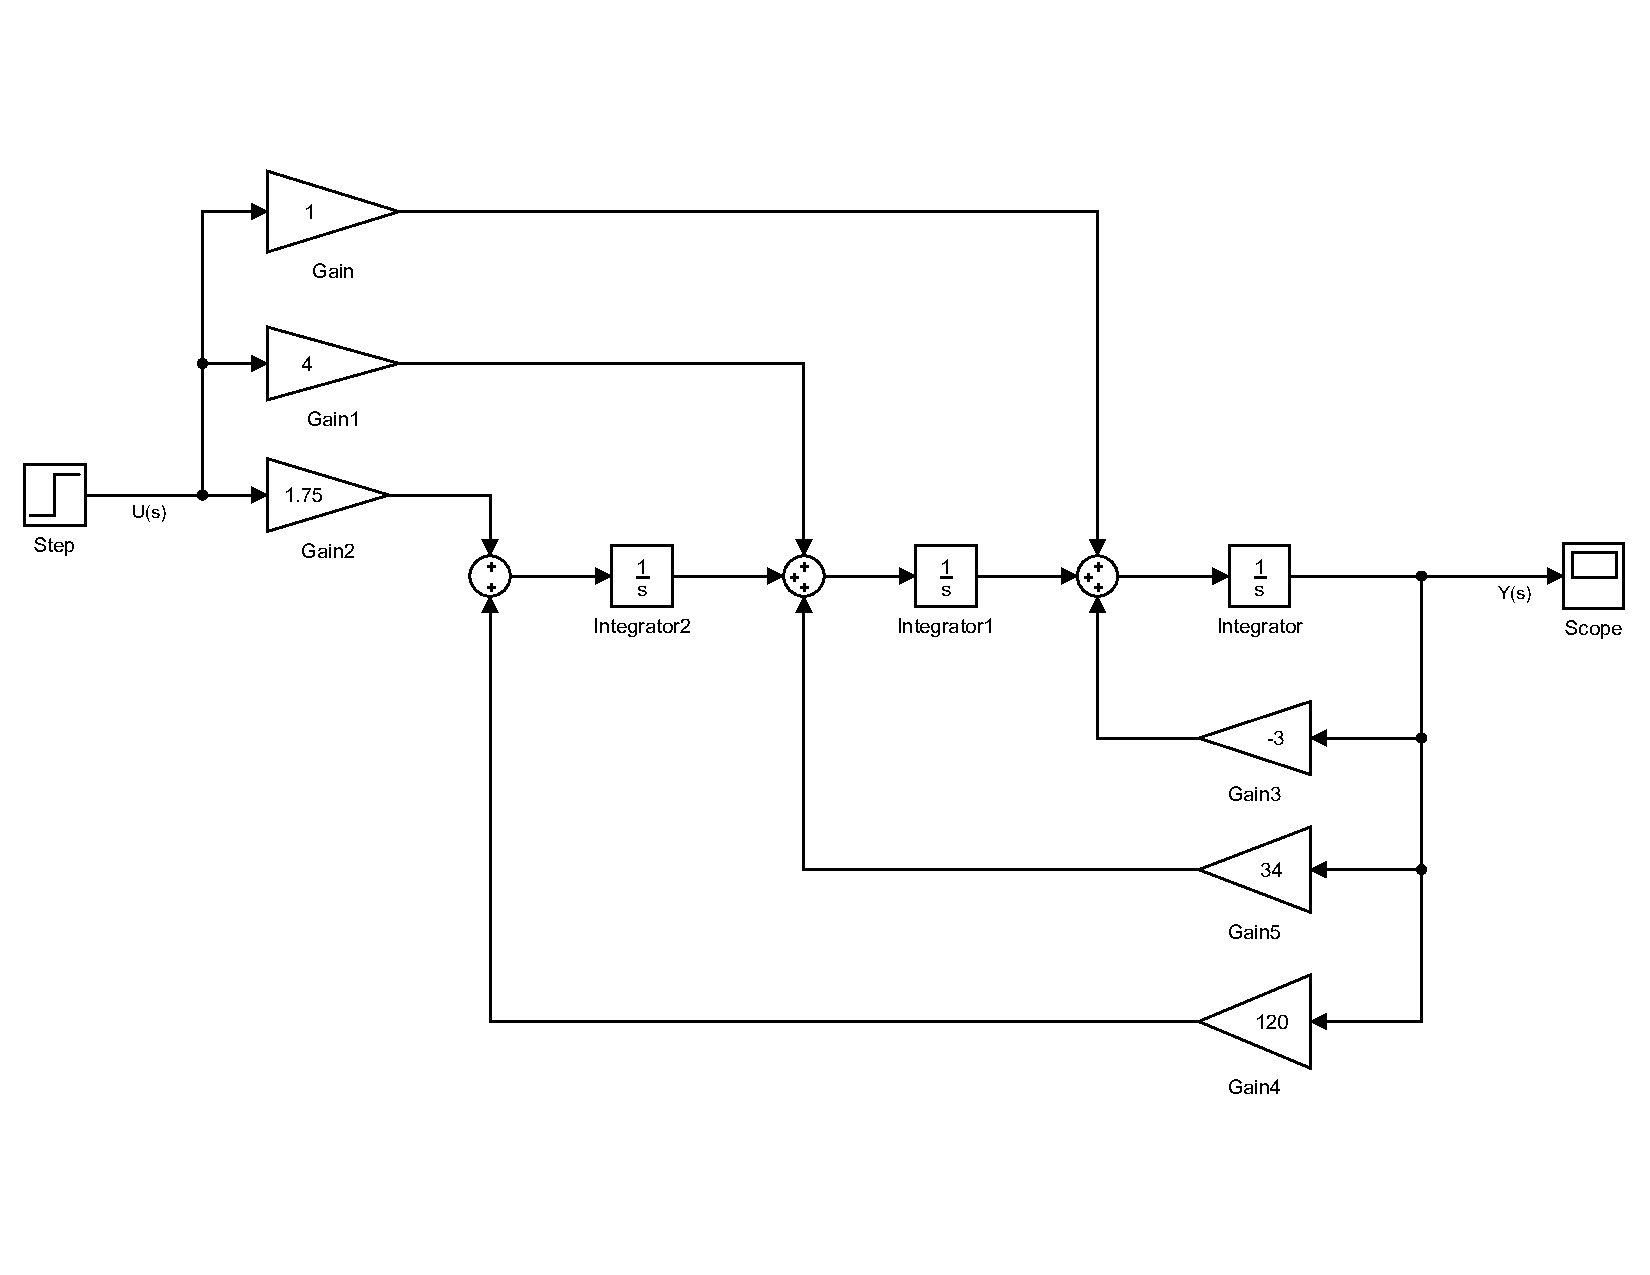
\includegraphics[width=0.9\linewidth]{Z1_2}
\caption{Reprezentacja graficzna modelu otrzymanego drugim wariantem metody bezpośredniej}
\label{fig:z12}
\end{figure}

\section{Zadanie 2 - Dowód, że oba warianty metody bezpośredniej dają tą samą transmitancję}
Dla modelu z pierwszego wariantu metody bezpośredniej mamy macierze postaci:
\[A_1 = \begin{bmatrix} -a_2 & -a_1 & -a_0\\ 1 & 0 & 0\\ 0 & 1 & 0 \end{bmatrix};
B_1 = \begin{bmatrix} 1\\ 0\\ 0 \end{bmatrix};
C_1 = \begin{bmatrix} b_2 & b_1 & b_0 \end{bmatrix};
D_1 = 0
\]

Dla modelu z drugiego wariantu metody bezpośredniej mamy macierze postaci:
\[A_2 = \begin{bmatrix} -a_2 & 1 & 0\\ -a_1 & 0 & 1\\ -a_0 & 0 & 0 \end{bmatrix};
B_2 = \begin{bmatrix}  b_2\\ b_1\\ b_0 \end{bmatrix};
C_2 = \begin{bmatrix} 1 & 0 & 0 \end{bmatrix};
D_2 = 0
\]

Dla wzoru 
\[G(s) = C(sI - A)^{-1}B + D\]

Otrzymujemy:
\[G_1(s) = G_2(s) = \frac{b_2s^{-1} + b_1s^{-2} + b_0s^{2}}{1 + a_2s^{-1} +a_2s^{-2} +a_0s^{-3}}\]
co należało dowieść

\section{Zadanie 3 - Porównanie odpowiedzi skokowej}
Dla \[x_0 = \begin{bmatrix}
0 & 0 & 0
\end{bmatrix}\]
wszytkie trzy modele jednakowo reagują na odpowiedz skokową. 

\section{Zadanie 5 - Sprawdzenie sterowalności o obserwowalności}
\[det(\begin{bmatrix}B_1 & A_1B_1 & A^2_1B_1\end{bmatrix}) = 
det(\begin{bmatrix} 1 & -3 & 43\\ 0 & 1 & -3\\ 0 & 0 & 1 \end{bmatrix}) = 1 \neq 0\]
Więc obiekt jest sterowalny.

\[det(\begin{bmatrix}C_1 \\ C_1A_1 \\ C_1A^2_1\end{bmatrix}) = 
det(\begin{bmatrix} 1 & 1 & \frac{131}{4}\\ 4 & \frac{143}{4} & 154\\ \frac{7}{4} & 120 & 120 \end{bmatrix}) = -729.4219 \neq 0\]
Więc obiekt jest obserwowalny.

\section{Zadanie 6 - Projektowanie układu regulacji}

\end{document}